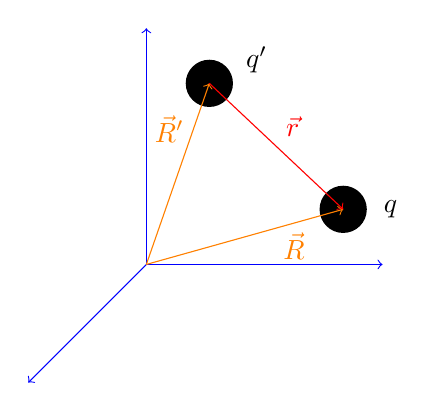
\begin{tikzpicture}
\node (C) at (0,0) {};
\draw [blue,->] (C.center)--(0,3);
\draw [blue,->] (C.center)--(3,0);
\draw [blue,->] (C.center)--(-1.5,-1.5);
\fill  (0.8,2.3) node (v1) {} circle (0.3);
\fill  (2.5,0.7) node (v2) {} circle (0.3);
\node at (1.4,2.6) {$q'$};
\node at (3.1,0.7) {$q$};
\draw [->,orange] (C.center) -- (v1.center) node [near end,left] {$\vec{R}'$};
\draw [->,orange] (C.center) -- (v2.center) node [near end,below] {$\vec{R}$};
\draw [->,red] (v1.center) -- (v2.center) node [midway,above right] {$\vec{r}$};
\end{tikzpicture}